
\documentclass[main.tex]{subfiles}

\begin{document}
\section{Грубо в мозъка}
\end{document}

\begin{figure}[H]%
    \centering
    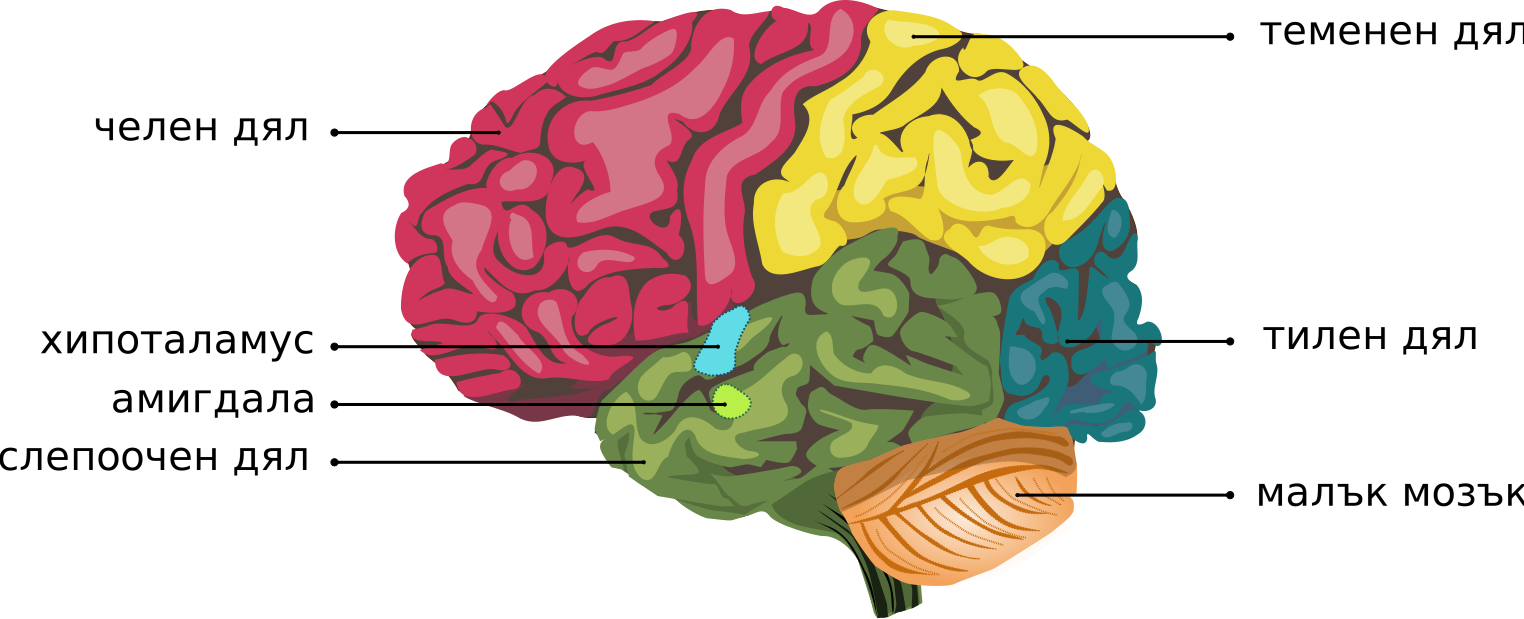
\includegraphics[width=0.8\paperwidth,valign=t]{brain}%
    \caption{Дялове на мозъка}%
    \label{fig:brain_physics:1}
\end{figure}
Нервната система се разделя на централна, състояща се от главен и гръбначен мозък, и периферна. Главната функция на нервната система е да контролира работата на тялото. Информацията от околната среда се събира чрез периферната система, предава се към централната, която взима решение за съответна реакция и изпраща обратно съобщение към периферната нервна система.

Невроните (нервни клетки) са базовата функционална единица на нервната система. Те са електрически възбудими и си предават информация посредством електрически сигнали, които се предават през специални връзки между тях - синапси. Електроенцефалографът измерва колебания в напрежението върху повърхността на скалпа чрез множество метални пластинки, наречение електроди, долепени до него от едната страна и свързани с кабел към уреда от другата. Сигналите, получени от електроенцефалографа, се групират по (полезни)честотни ленти по следния начин:

\begin{itemize}
    \item $(1-4Hz) \delta$ вълни

    Асоциират се с така наречения бавновълнов сън\footnote{NREM - non-rapid eye movement sleep}, тоест най-дълбоката фаза на съня.
    \item $(4-8Hz) \theta$ вълни

    Има два вида $\theta$ вълни. Едните се засичат в хипокампа (частта от мозъка, свързана с формирането на спомени) и произходът им не е съвсем ясен, има разнообразни изследвания с плъхове, които изследват този вид $\theta$-ритъм.
    Другите се наричат корови и са свързани с фазата на оживено сънуване\footnote{REM - rapid eye movement sleep. Също така чудесна музкална група}.

    \item $(8-12Hz) \alpha$ вълни

    Това е най-добре изучената честотна лента. Асоциират се със спокойно будно състояние със затворени очи.

    \item $(13-30Hz) \beta$ вълни

    $\beta$ вълните се асоциират с нормално будно състояние.
    \item $(30-50Hz)\gamma$ вълни (ниски)

    Според проучвания, те се свързват с изострено внимание, работеща краткосрочна и дългосрочна памет.
\end{itemize}

Главното действие на централната нервна система се осъществява в мозъчната кора, която обхваща $40\%$ процента от обема на главния мозък. Мозъчната кора се дели на няколко дяла:

\begin{itemize}
    \item Челен дял

    Този дял се свързва с всякакви когнитивни умения. Отговорен и за моторните функции - тоест умението да движим мускулите си доброволно.
    \item Теменен дял

    Той е отговорен за приемането и съчетаването на сетивна информация. Главната му функция се описва с действието ,,диференциране на две точки'' - това е възможността на мозъка да различи, че два отделни предмета, докосващи кожата, са наистина различни, а не един.


    По този начин теменният дял участва в съставни действия като разпознаване на лица и сцени.

    \item Тилен дял

    Тилният дял е отговорен за зрението - разпознава заобикалящата среда, детайли и цветове в нея. В тилния дял се определя ,,какво'', ,,къде'' и ,,как'' вижда човек.


    \item Слепоочен дял

    Слепоочният дял се състои от структури, които са важни за дългосрочната памет. В него се намира хипокампа, който е главният дял, отговарящ за спомените. Амигдалата също е част от слепоочния дял, макар че се намира по-навътре. Смята се, че тя е отговорна за формиране на емоционален отговор, като е особено обвързана с негативните емоции.
\end{itemize}

Освен на дялове, разглеждаме деленето на мозъчната кора на ляво и дясно полукълбо.

При измерването на напрежението с енцефалограф, се откриват различни модели на емоциите, в зависимост от енергията на $\theta, \beta, \alpha, \gamma$ вълните в определени дялове на мозъка.

Например по-голяма активация на $\alpha$-вълни в дясната част на челния дял се свързва със стимули, които карат човек да ,,бяга'' (от инстинкта ``бий се или бягай''), тоест отговаря за негативни емоции като ,,погнуса'' и ,,страх''.
По-голяма активност на $\alpha$-вълни в ляво на челния дял се асоциира с позитивни стимули и емоции. Това означава, че асиметрията на челния дял говори за разлика във валентността. Смята се, че $\beta$ и $\gamma$ вълните също носят информация за валентността на емоцията. Например, при позитивни емоции $\gamma$ вълните в слепоочния дял почти отсъстват, докато са с висока мощност при негативни емоции.

Активирането на амигдалата, както споменахме, също е свързано с негативни емоции. Често я наричат ,,зона на страха'' \footnote{поетично}.

Топлограмата от \autoref{fig:brain_physics:2} показва разликата между енергиите на $\theta, \beta, \alpha, \gamma$ вълните, измерени от различните електроди, за всяка една от емоциите. Графиката е направена подобно на тези в \cite{heatmap}. В това изследване се цели да се намерят стабилни шаблони на емоции в ЕЕГ сигнала. Опитът се провежда върху едни и същи субекти в различен момент от време, като се разпознават четирите квадранта на активация-валентност пространството. Показва се, че активните сектори не се променят през времето.
\begin{figure}[H]%
    \centering
    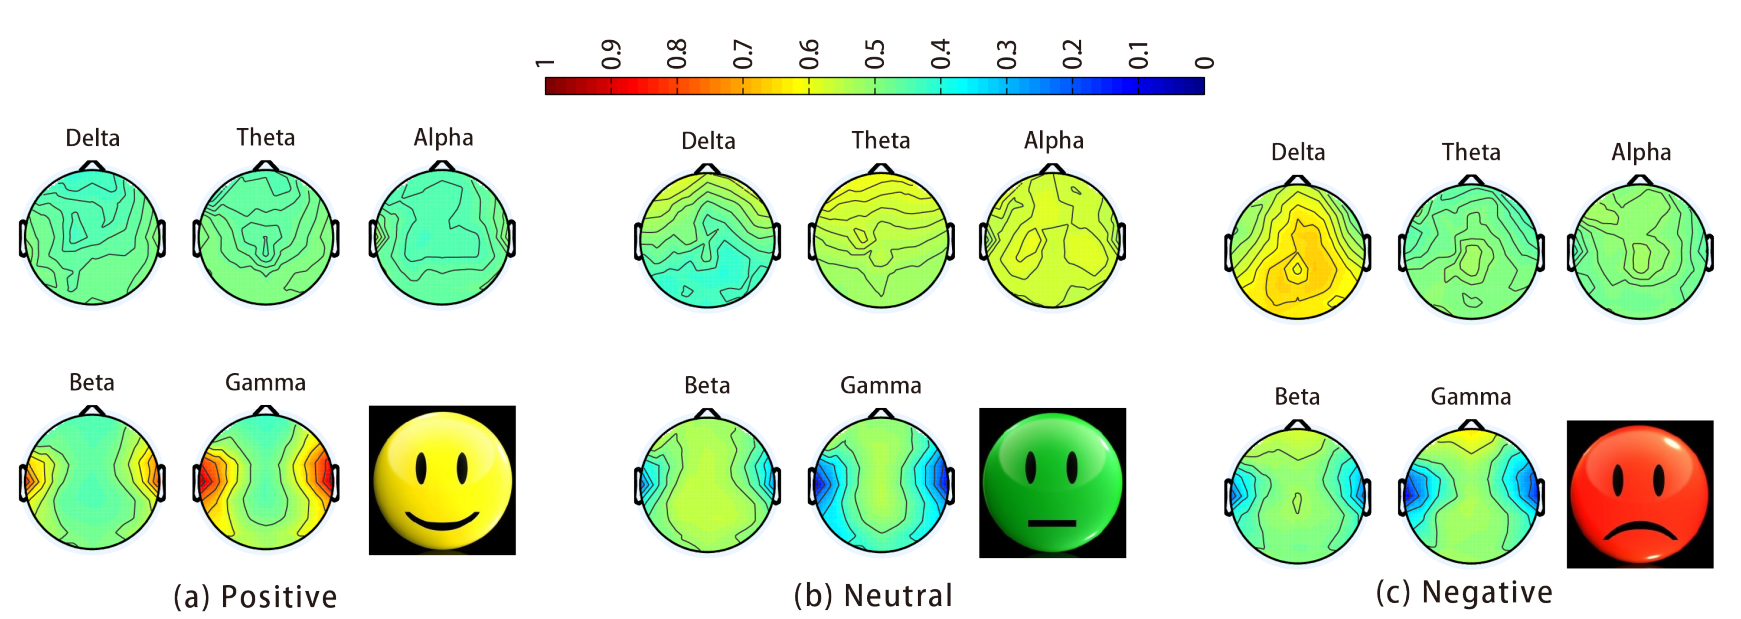
\includegraphics[width=0.8\paperwidth,valign=t]{emotion_map.png}%
    \caption{{\small Топлограма на емоциите.} Всяка една от вълните е нормализирана върху всички емоции. Червено значи висока активност, а синьо - ниска.}%
    \label{fig:brain_physics:2}
\end{figure}

Следователно, бихме искали да изследваме енергията на $\theta, \delta, \alpha, \beta, \gamma$ вълните в различните дялове на мозъка.
